\chapter{Evaluation and Results}
This chapter will first explain the configuration and results of the experiments used to determine the vocabulary size (Section \ref{sec:4-vocab_size}) and sentence length (Section \ref{sec:4-sentence_length}). Following this are details of experiments for the Baseline model (Section \ref{sec:4-baseline}), Trivial Transfer Learning model (Section \ref{sec:4-trivial}), and Hierarchical Transfer Learning model (Section \ref{sec:4-hierarchical}).
\newpage

\section{Experiments}

The Scottish Gaelic dataset consists of 145,000 sentences from the the original and back-translated data, as described in Table \ref{tab:low_resource-data}. The French dataset consists of 170,000 sentences from the data described in Table \ref{tab:available-data}. Finally the Irish Gaelic dataset consists of 165,000 sentences from the back-translated monolingual English data extracted from the Italian and Spanish data described in Table \ref{tab:available-data}.
All of the sentences fit within the maximum sentence length of 20 words and as mentioned in the methodology.
For the parent and intermediary languages, the test split been set to 0 and the validation split has been set to 0.1. This means that a significantly higher percentage of the available sentences are used for training. In line with the existing transfer learning research identified in the literature review, parent models were trained for 5 epochs before switching the dataset to child languages.

% ======================================================

\subsection{Vocabulary Size}
\label{sec:4-vocab_size}

During data pre-processing, the source and target language vocabulary size have been limited, with prioritisation given to the most frequently occurring words. To determine the most suitable vocabulary size for the full Scottish Gaelic dataset with 145,000 sentences, tests at sizes 4000, 5000, and 7000 were completed. Due to the total vocabulary size with a minimum word occurrence of 2 totalling approximately 7000, the maximum possible size for this dataset is 7000. 
The vocabulary size of subsequent experiments will be determined by selecting the vocabulary size that returns highest \acrshort{BLEU} score. The validation loss during training and \acrshort{BLEU} score of each size is shown in Figure \ref{fig:vocab_loss_bleu}.

\begin{figure}[ht!]
\centering
\makebox[\textwidth][c]{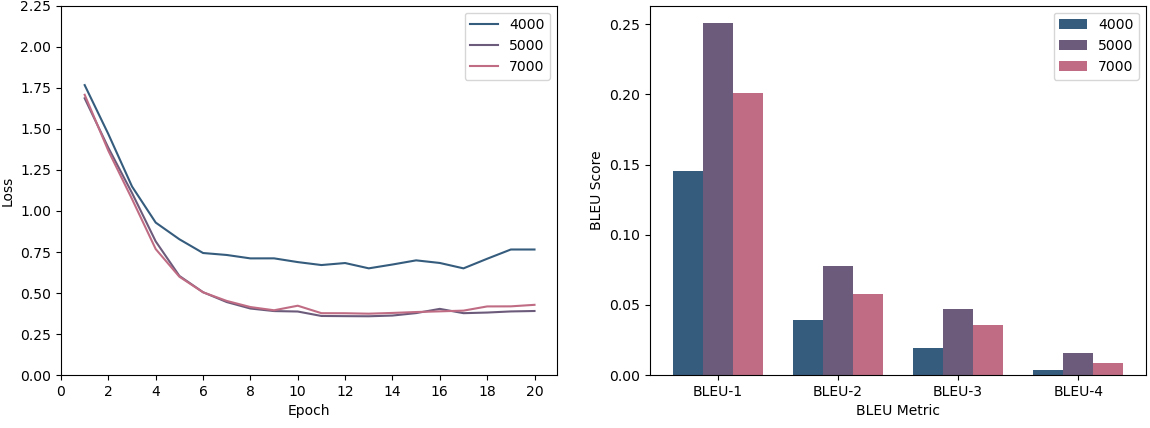
\includegraphics[width=1.15\textwidth]{media/experiments/bleu/vocab_loss_bleu.jpg}}
\captionsetup{justification=centering}
\caption[Vocabulary size experiment validation loss and BLEU score]{Vocabulary size experiment. Left: Validation loss. Right: BLEU score}
\label{fig:vocab_loss_bleu}
\end{figure}

Despite similar validation loss values between 5000 and 7000, the highest \acrshort{BLEU} scores were achieved when the vocabulary size was 5000. The \acrshort{BLEU} score of each vocabulary size is proportional to each other for each n-gram count with a ratio of approximately $3:5:4$ for values 4000, 5000, and 7000. 

% ======================================================

\subsection{Sentence Length}
\label{sec:4-sentence_length}

As mentioned previously, padding is added to any sentence with less words than the longest sentence. To determine the most suitable sentence length for the Scottish Gaelic dataset, tests at sizes 15 and 20 were completed. These values were selected based on the analysis of the dataset in Figure \ref{fig:sentence_length-gaelic}, where the majority of sentences fall within a 15 word limit, with an additional 6,000 sentences between 16 and 20. This experiment will reveal whether a reduction in the overall variable length sequence padding improves the translation quality.
139,000 sentences from the Scottish Gaelic dataset were used for both sizes, using the vocabulary size of 5000 as determined by the result of the previous experiment. Subsequent experiments will use the sentence length that the yields highest \acrshort{BLEU} score. The validation loss and \acrshort{BLEU} score of each sentence length is shown in Figure \ref{fig:length_loss_bleu}.

\begin{figure}[ht!]
\centering
\makebox[\textwidth][c]{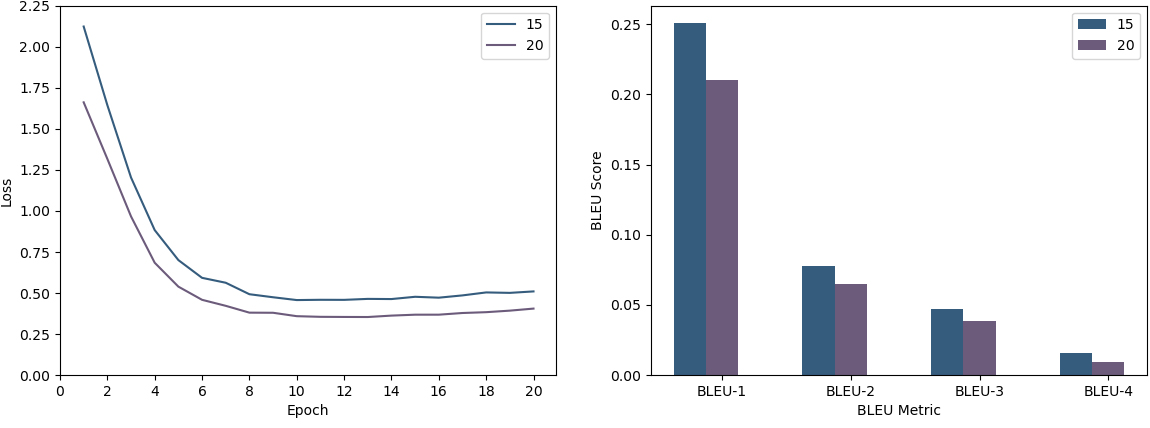
\includegraphics[width=1.15\textwidth]{media/experiments/bleu/length_loss_bleu.jpg}}
\captionsetup{justification=centering}
\caption[Sentence length experiment validation loss and BLEU score]{Sentence length experiment. Left: Validation loss. Right: BLEU score}
\label{fig:length_loss_bleu}
\end{figure}

While a sentence length of 20 resulted in a lower validation loss during training, the \acrshort{BLEU} score evaluation shows that a sentence length of 15 results in a better translation quality. The maximum \acrshort{BLEU} score for a length of 15 is 0.25 \acrshort{BLEU}, compared to a maximum of 0.21 \acrshort{BLEU} for a length of 20. This is approximately the same difference in \acrshort{BLEU} score as the top two choices vocabulary size, suggesting that the impact of selecting the highest scoring vocabulary size and sentence length for the remaining experiments will have a significant impact on the results. 

% ======================================================

\subsection{Baseline}
\label{sec:4-baseline}

The baseline translation model described in Section \ref{sec:3-model} has been trained for 20 epochs with a vocabulary size of 5000 using 139,000 sentences from Scottish Gaelic dataset with a maximum sentence length of 15. The training and validation loss can be seen in Figure \ref{fig:loss_baseline}.

\begin{figure}[ht!]
\centering
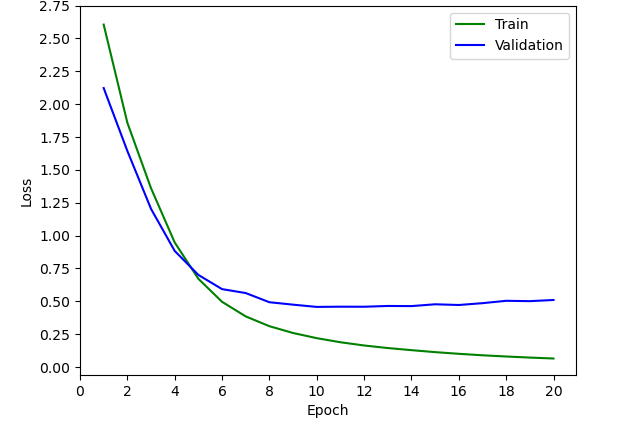
\includegraphics[width=0.75\textwidth]{media/experiments/loss/5k/loss_baseline.png}
\captionsetup{justification=centering}
\caption[Baseline model training and validation loss]{Baseline model training and validation loss}
\label{fig:loss_baseline}
\end{figure}

The baseline model achieved the lowest validation loss during epoch 10 with a value of 0.457. Subsequently, the validation loss slowly increased over time for the remaining 10 epochs as the model began overfitting on the training set. For comparison with other models in subsequent experiments, the translation evaluation is available at end of this chapter in Section \ref{sec:4-results}.

% ======================================================
\newpage
\subsection{Trivial Transfer Learning}
\label{sec:4-trivial}

The trivial transfer learning method that is described in Section \ref{sec:2-transfer_learning} has been implemented using a vocabulary size of 5000 and maximum sentence length of 15 using 170,000 sentences from the French dataset as the parent language and 139,000 sentences from the Scottish Gaelic dataset as the child language. The parent language was trained for 5 epochs, initialising the child language that was trained for a further 15 epochs. The training and validation loss is shown in Figure \ref{fig:loss_trivial}.

\begin{figure}[ht!]
\centering
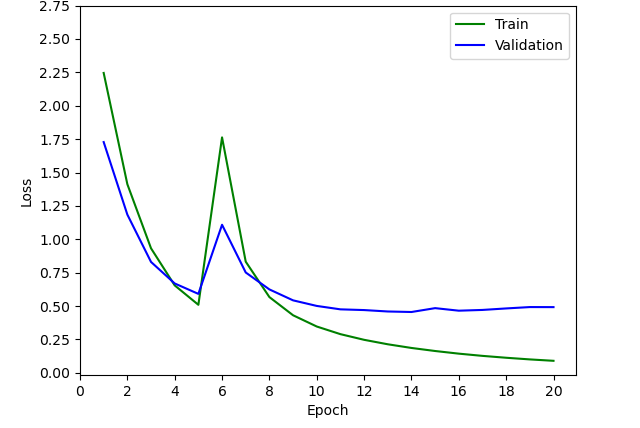
\includegraphics[width=0.75\textwidth]{media/experiments/loss/5k/loss_trivial.png}
\captionsetup{justification=centering}
\caption[Trivial transfer learning model training and validation loss]{Trivial transfer learning model training and validation loss}
\label{fig:loss_trivial}
\end{figure}

As observed in Figure \ref{fig:loss_trivial}, a spike in both the training and validation loss of the model is present after 5 epochs. This is a result of switching from the French parent dataset to the Scottish Gaelic child dataset. The lowest validation score achieved in this model during training on the Scottish Gaelic data was 0.455, 0.002 lower than the baseline model.
% This is 0.002 points lower than the best validation loss observed in the baseline model.

% ======================================================


\subsection{Hierarchical Transfer Learning}
\label{sec:4-hierarchical}

The hierarchical transfer learning approach described in Section \ref{sec:2-transfer_learning} has been implemented using French as the parent language, Irish Gaelic as the intermediary language and Scottish Gaelic as the child language. Both the French dataset and Irish Gaelic dataset include 170,000 sentences. The French parent was trained for 5 epochs, then the data was switched to Irish Gaelic and trained for another 5 epochs before finally training on Scottish Gaelic data for 12 epochs. The training and validation loss is shown in Figure \ref{fig:loss_hierarchical}.

\begin{figure}[ht!]
\centering
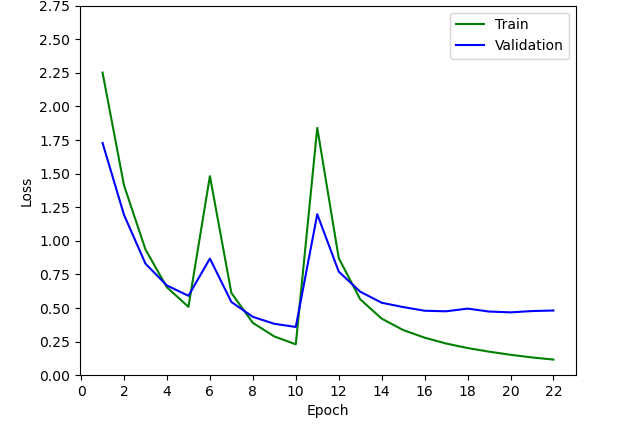
\includegraphics[width=0.70\textwidth]{media/experiments/loss/5k/loss_hierarchical.png}
\captionsetup{justification=centering}
\caption[Hierarchical transfer learning model training and validation loss]{Hierarchical transfer learning model training and validation loss}
\label{fig:loss_hierarchical}
\end{figure}

Spikes in both the training and validation loss are observed at epoch 5 and 10, where the dataset has been switched between languages. The lowest validation loss was achieved after training for 10 epochs on the Scottish Gaelic dataset with a value of 0.467 on epoch 20. This is significantly higher than the lowest validation loss observed during the training of the intermediary Irish Gaelic dataset which reached a value of 0.358 after only 5 epochs.

% ======================================================

\newpage
\section{Results}
\label{sec:4-results}

A comparison of the \acrshort{BLEU} score evaluations collated from the experiments using the baseline model (Section \ref{sec:4-baseline}), trivial transfer learning model (Section \ref{sec:4-trivial}), and hierarchical transfer learning model (Section \ref{sec:4-hierarchical}) are shown in a bar chart in Figure \ref{fig:bleu_results}.

\begin{figure}[!ht]
\centering
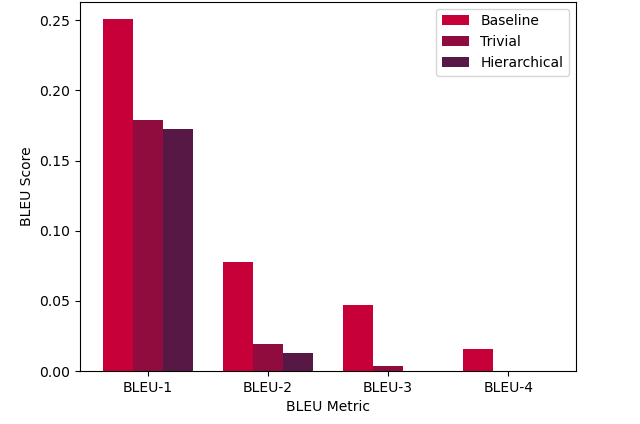
\includegraphics[width=0.75\textwidth]{media/experiments/bleu/5k_bleu.png}
\captionsetup{justification=centering}
\caption[Model BLEU scores]{Model BLEU scores}
\label{fig:bleu_results}
\end{figure}

The bar chart demonstrates the significant difference in \acrshort{BLEU} scores between the baseline and transfer learning models. The baseline model consistently scores higher in all \acrshort{BLEU} score n-gram counts, with the highest being approximately 0.25 \acrshort{BLEU} for \acrshort{BLEU}-1. For both \acrshort{BLEU}-3 and \acrshort{BLEU}-4, hierarchical transfer learning achieved a \acrshort{BLEU} score of 0, with trivial transfer learning scoring very close to 0 on \acrshort{BLEU}-3 and 0 on \acrshort{BLEU}-4. The exact values for each experiment are shown in Table \ref{tab:bleu_table}, along with an additional \acrshort{NIST} translation evaluation metric.


\begin{table}[!ht]
\centering
\setlength\doublerulesep{2pt}
\renewcommand{\arraystretch}{1.1}
\begin{longtable}{|l|l|l|l|l|l|}
\hline
\textbf{Model} & \textbf{BLEU-1} & \textbf{BLEU-2} & \textbf{BLEU-3} & \textbf{BLEU-4} & \textbf{NIST}\\ \hline
\endhead
%
\hline
\endfoot
%
\endlastfoot
%
Baseline       & 0.2507 & 0.0775 & 0.0469 & 0.0157 & 1.1978 \\
Trivial        & 0.1789 & 0.0196 & 0.0033 & 0.0004 & 0.7698 \\
Hierarchical   & 0.1723 & 0.0133 & 0.0000 & 0.0000 & 0.7814 \\ \hline
\captionsetup{justification=centering}
\caption{Translation evaluation scores}
\label{tab:bleu_table}\\
\end{longtable}
\end{table}

The \acrshort{BLEU} scores of Table \ref{tab:bleu_table} suggest that the quality of trivial transfer learning is slightly better than hierarchical transfer learning. In contrast, the \acrshort{NIST} evaluation metric implies that the translation for hierarchical transfer learning marginally outperforms trivial transfer learning. The source and reference sentence from two cleaned samples in the test set are shown in Table \ref{tab:sentence_analysis}, including the translation that each model provided for that sentence.


\begin{table}[!ht]
\centering
\setlength\doublerulesep{2pt}
\renewcommand{\arraystretch}{1.1}
\begin{tabular}{|l|p{7cm}|}
\hline
\multicolumn{2}{|l|}{\textbf{Scottish Gaelic \textrightarrow \space English Translation}} \\ \hline
Source          & an t eun a tha marbh \\ \hline
Reference       & the bird is dead \\ \hline
Baseline        & the unk is the unk \\ \hline
Trivial         & are nothing t a would is \\ \hline
Hierarchical    & he don a would this to is \\ \hhline{==}
Source          & tha e na chadal   \\ \hline
Reference       & he s asleep   \\ \hline
Baseline        & the unk is the unk   \\ \hline
Trivial         & he in a him would lot are nothing \\ \hline
Hierarchical    & he in a   \\\hline
\end{tabular}
\captionsetup{justification=centering}
\caption{Translation sentence analysis}
\label{tab:sentence_analysis}
\end{table}

The sentence analysis table reveals the poor translation quality that lead to such low \acrshort{BLEU} scores. The samples also show that the baseline model is consistently outputting very similar sentences that include common words, potentially influencing the evaluations.